%% FELthesis: LaTeX class for bachelor, master, and phd thesis in CTU FEL
%% template.tex: template file
%% (c) 2012-2014 Vít Zýka, vit.zyka@seznam.cz
%%
%% 2012-12-17 v0.1 first version derived from cmpthesis.tex

\documentclass[bcl,czech]{felthesis} % or 

%% --- your additional packages:
\usepackage[utf8]{inputenc}

%% --- usefull draft packages
\usepackage[notref]{showkeys} % show labels for referencies
%%\usepackage{showlabels}       % similar
%%\usepackage{showidx}          % show index entries on every page
%\usepackage{fancyhdr}
%\usepackage{graphicx} 
%\usepackage{epstopdf}
%\usepackage{cuted}
\usepackage{amsmath}

%% ======================================================== thesis info
\startThesisInfo
  \Title{ Hidden }%Ovládání robotu sledujícího člověka gesty}
  \Author{ Hidden }
  \Date{Červen 2018}
  \Department{ Hidden }
  \Advisor{ Hidden }
  \KeywordsCz{První klíčové slovo; druhé; třetí; \dots}
  \KeywordsEn{First keyword; second; third; \dots}
  %\AssignmentPage{assignment.pdf} % insert official assignment if given
\stopThesisInfo

%% ============================== your definitions (abbreviations etc.)
%%\def\Ax{\mathbf{A}_{x}}

%% =========================================================== settings
\addbibresource{\jobname.bib} % bibliography file

\graphicspath{{fig/}{logo/}} % subdirectories where TeX finds pictures

%% ========================================================== text body
\begin{document}

\MakeTitle

\startFrontMatter
  \startAcknowledgement
Text of acknowledgement\dots
\stopAcknowledgement

\endinput
%%
%% End of file `acknowledgement.tex'.

  \startDeclaration
\ifCzech
  Prohlašuji, že jsem předloženou práci vypracoval samostatně,
  a~že jsem uvedl veškeré použité informační zdroje v~souladu
  s~Metodickým pokynem o~dodržování etických principů při přípravě
  vysokoškolských závěrečných prací.
\fi
\ifEnglish
  I declare that I worked out the presented thesis independently
  and I quoted all used sources of information in accord with
  Methodical instructions about ethical principles for writing
  academic thesis.
\fi
\stopDeclaration

\endinput
%%
%% End of file `declaration.tex'.

  \startAbstractCz
%shrnutí celé práce
%popisný abstrakt vysvětluje účel, cíl a metody 100-200 slov
%proč jste se rozhodli psát na toto téma? proč je tenhle "výzkum" důležitý?
%metody
%výsledky?

%    Čím se v textu práce zabýváte (jakým problémem)?
%    Jaké metody jste použili na zjištění / výzkum / řešení problému?
%    Jakých výsledků jste dosáhli?


Tato práce řeší detekci ruky pomocí kamery Kinect a rozpoznávání gest. Cílem této práce je vytvořit podklad pro řízení robotu, který bude interagovat s člověkem. Zaměřila jsem se na charakteristické rysy ruky a rozpoložení prstů.
Práce představuje algoritmus, který využívá pouze euklidovské vzdálenosti. Data z kamery jsem zpracovávala pomocí openFrameworks s využitím doplňku ofxKinectV2.

%Podstatou našeho algoritmu je.

%Podařilo se dosáhnout úspěšnosti 87,3%.
%V práci jsme vytvořili systém, který.
%Vytvořené řešení poskytuje ty a ty možnosti.
%Provedeným výzkumem jsme zjistili, že.

%Přínosem této práce je.
%Hlavním zjištěním je.
%Hlavním výsledkem je.
%Na základě zjištěných údajů je možné.
%Výsledky této práce umožňují.
\stopAbstractCz

\startAbstractEn
This thesis deals with hand detection and gesture recognition from video stream captured by Kinect camera. The aim of thesis is to create data to control robot for human-robot interaction. Focus was on features of the hand and fingers. Thesis presents an algorithm based on euclidean distances. Data was processed using openFrameworks software with ofxKinectV2 addon.
\stopAbstractEn

\endinput
%%
%% End of file `abstract.tex'.

  \TableOfContents
  \startAbbreviations{%
  Preliminary text\dots
}

\abbrv[OF]	openFrameworks \dots nástroj pro kreativní programování
\abbrv[FBO]  "frame buffer object" \dots objekt pro vykreslování v OF
\abbrv[HMM]  "Hidden Markov Model" \dots Skrytý Markovův model
\abbrv[P2DHMM]  "Pseudo-2D Hidden MArkov Model
\abbrv[VR]  virtuální realita
\abbrv[DOF]  "degree of freedom" \dots stupeň volnosti
\abbrv[SVM]  "support vector machines" \dots metoda podpůrných vektorů
\abbrv[ToF]  "Time-of-Flight" \dots doba letu aneb hloubkové kamery založené na výpočtu vzdálenosti z doby letu laseru
\abbrv[ROI]  "Region of interest" \dots oblast zájmu
\abbrv[RBF]  "Radial Basis Functions"

\abbrv[...]     ...
\stopAbbreviations

\endinput
%%
%% End of file `abbreviations.tex'.

\stopFrontMatter

\startBodyMatter
  %\includeonly{ch01}
  \chapter{Úvod}
%-full-textové vyhldávání (key-words?)
%seznámení s problematikou - současná situace, motivace
V dnešní době robotizace, kdy lidé přicházejí na výhody využívání inteligentních zařízení, je snaha rozšířit jejich využití co nejvíce. Ovládání gesty značně pomůže intuitivnímu řízení robotů a usnadní jejich využití.
Z pohledu spolupráce běžného uživatele s robotem se řadí řízení zařízení za pomoci kamery mezi nejjednodušší způsoby, jelikož kamery jsou relativně levné a dostupné. Není k tomu potřeba nic jiného, než co většina populace (alespoň cílové skupiny - lidí používajívící počítače) už má. Jedná se o jednodušší variantu i s ohledem na implementační čas.

Mnoho podobných aplikací již existuje, nebo se zaměřuje na jednotlivé podčásti, často ale vyžadují složitou instalaci a konfiguraci programů. Velké množstí pak ani nepodporuje zpracování s malou časovou odezvou a jsou výpočetně složité a časové náročné.
%cíle BP
Jelikož má být výsledný algoritmus použitelný pro robota, který  bude  následovat člověka, musí splňovat několik požadavků. Jedná se o systém reálného času a tam musí být odezva dostatečně malá s ohledem na člověka. Zvolená gesta musí být intuitivní a snadno proveditelná. 		%další požadavky 

%odůvodnění proč a jak
Následně zvolené přístupy v této práci jsou psány tak, aby měly co nejmenší odezvu. 
V aktuálních aplikacích se obvykle využívají strojově naučené algoritmy. Pro snazší dosáhnutí rychlejšího zpracování obrazu, které vyhovuje požadavkům, lze využít vlastností obrazu, jako jsou vzdálenosti a úhly k rozpoznávání ruky.
%popsání logického členění BP



\endinput
  \textit{}\chapter{Stávající metody a aplikace}
%Some introductory text\dots

\section{Stávající metody}
\subsection{Předzpracování obrazu}
\subsubsection{Binární obraz}
Většina metod se zakládá na zpracování binárního obrazu. Probíhá to zvolením prahové hodnoty, se kterou se všechny hodnoty porovnají a ve výsledku vznikne binární obraz. Objekt, který je středem zájmu, se skládá z pixelů s hodnotou 1 zatímco ostatní mají hodnotu 0.
\subsubsection{Rozostření}
Rozostření slouží k eliminaci šumu v obraze. Nejosvědčenější metody jsou nízkofrekvenční filtry jako je Gauss a medián. Tato kapitola čerpá z Pikoly~\cite{15} kapitoly 5 a 6.\\

Filtr medián se zaměřuje na vyhlazování lokálních extrémů z obrazu. Nezachovává jemné čáry a ostré rohy, takže je vhodný pouze v aplikacích, kde na tom nezávisí aplikace. Výraznou výhodu představuje v odstranění extrémů, které v obraze mohou vzniknout. Narozdíl od průměrování obraz nezkreslí chybné pixely s extrémníma hodnotama. % Nejprve se seřadí všechny hodnoty z aktuální konvoluční matice a vybere hodnotu, která leží uprostřed seřazeného pole a tou nahradí zpracovávaný bod.
 
Velikost okolí zahrnutého v analýze se může zvětšit při větší hustotě šumu. V aplikaci na hloubkový obraz, ve kterém se detekují prsty je ale důležité zachovat určité rozlišení. Na obrázku 1 lze pozorovat rozdíly mezi filtrem s průměrováním (b) a mediánem (c).\\

\begin{figure}[h]
\centering
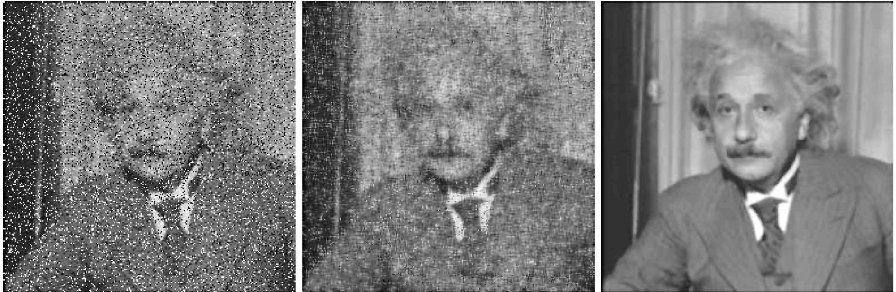
\includegraphics[width=0.8\linewidth]{median.jpg}
\caption{a) původní obraz b) průměrování c) medián\\
 Převzato z ~\cite{15} }
\end{figure}

\newpage
Gaussovský filtr je průměrování s Gaussovským rozložením. Využívá se k vyhlazování obrazu a odstranění detailů a šumu. Obrázek 2 zachycuje rozdál mezi opakovanou aplikací Gaussovského filtru.
\begin{eqnarray}
G(x,y) = \frac{1}{2 \pi \sigma^{2}}*e^{-\frac{x^{2}+y^{2}}{2\sigma^{2}}}  ,
%ae^{-\frac{(x-b)^{2}}{2c^{2}}}
\end{eqnarray}
kde x a y jsou souřadnice a $ \sigma $ je směrodatná odchylka.\\

Aby se zabránilo rozšíření do nekonečna se v konvoluční masce přidělí větší váha bodu ve středu. Aby se aplikací konvoluční masky neměnila světlost, součet všech složek konvoluční matice dává hodnotu 1. Příklad konvoluční masky:
\begin{eqnarray}
\frac{1}{16} \begin{bmatrix}
1 & 2 & 1 \\
2 & 4 & 2 \\
1 & 2 & 1
\end{bmatrix}
\end{eqnarray} 

\begin{figure}[h]
\centering
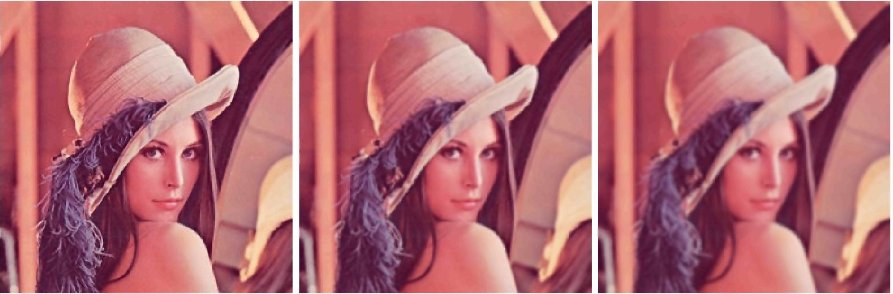
\includegraphics[width=0.8\linewidth]{gauss.jpg}
\caption{a) původní obraz b) jednou aplikovaný Gaussův filtr c) třikrát aplikovaný Gaussovský filtr
Převzato z ~\cite{15} }
\end{figure}

Mezi vysokofrekvenční filtry, které se používají na zpracování digitálního obrazu patří i Laplaceův filtr. Ve výpočtu se užívá gradient, což je vektorová veličina určující směr a strmost největšího růstu funkce. Laplaceův filtr využívá pouze velikost a pro její odhad se používá všesměrný operátor vycházející s parciálních derivací. %POPIS VYUZITI, PROC JE ZMINEMN?
%http://soc.nidv.cz/data/2007/01-2.pdf ?
\begin{eqnarray}
\nabla^{2}g(x,y) = \frac{\delta^{2}g(x,y)}{\delta x^{2}} + \frac{\delta^{2}g(x,y)}{\delta y^{2}}
\end{eqnarray} 
Laplacián je aproximován diskrétní konvolucí. Příklad konvolučního jádra:
\begin{eqnarray}
\begin{bmatrix}
0 & 1 & 0 \\
1 & -4 & 1 \\
0 & 1 & 0
\end{bmatrix}
\end{eqnarray} 


\subsection{Rozpoznávání postav}
Možnosti:

podle tvaru
\begin{itemize}
\item na základě modelu


\item na základě prvků

\item strojově naučené programy
\item neuronové sítě %-radial basis funkction
\item transformační matice vzdálenostních funkcí (chamfer)
\end{itemize}

podle barvy
\begin{itemize}
\item strojově naučené programy\\
\end{itemize}


Jednou z metod je dle Ch. Nakajima a spol.~\cite{6} ukládání několika obrázků, z nichž se detekuje pohybující se objekt a vše, co se nehýbe se označí za pozadí a ignoruje. Následně se naleznou kraje možné postavy, aby se vylepšil výsledek a vymazal šum. Pokud se jedinec pohybuje v druhém kroce, oříznutí probíhá z posledního získaného obrazu. Pokud nebyl detekován žádný jedinec, tak se do paměti uloží pozadí, které se z následujících obrazů rovnou vymaže pro větší přesnost. K vlastní identifikaci se použila SVM (support vector machines) a k-NN klasifikátor.\\

Hussein a spol.~\cite{9}používají k rozpoznání postavy prohledávání obrazu a porovnávání siluet s databází, ve které jsou vzory lidských postav. Shoda je detekována pomocí zkosením objektů. Vzory jsou ve formě binárního obrazu. Vzdálenost D mezi vzorem V a objektem z obrazu O se počítá vzorcem\\

\begin{eqnarray}
 D(O,V) = \frac{1}{|V|}\sum_{i}^{}C_{i}V_{i}   ,
\end{eqnarray}

kde |V| je počet pixelů v siluetě ve vzoru, $ T_{i} $ je hodnota pixelu $ i $ ve vzoru a $ C_{i} $ je rozdíl zkosení pixelu $ i $ v obraze. Čím menší hodnota mezi vzorem a obrazem, tím lepší shoda je detekována.
%// (patří do nového odstavce?)

Nalezení podobnosti zkosením předpokládá již nalezené hrany objektů v obraze. Vzor se překryje co nejvíce na objekt a transformací bodů jednoho objektu pomocí parametrických transformačních rovnic.\\

Jiný přístup poskytuje nalezení objektu v zorném poli pomocí hloubkové kamery, následným rozhodnutím, zda objekt má lidské nohy, nebo aspoň dva objekty odpovídající tvaru, a pokud ano, tak se přejde k dalšímu kroku, ve kterém se detekuje barva kůže z RGB vstupu. Nalezený výsledek slouží jako oblast k detekci obličeje, čímž je definitivně nalezen člověk~\cite{10}.\\

Gavrila ~\cite{7} se snaží snížit výpočetní náročnost tak, že nahrazuje procházení obrazu postupně schopností zaměřit se na jeden úryvek přímo a ve druhém kroce teprve hledá podobnosti tvarů. Dosahuje tak zpracování v reálném čase.
%These pixel values form a distribution of distances of the template features to the nearest features in the image
Shodu podle tvaru detekuje pomocí vzdálenosti křivek, která se počítá podobně jako u Hussein a spol.~\cite{9} 

\begin{eqnarray}
 D(O,V) = \frac{1}{|V|}\sum_{t\in T}^{}d_{I}(t) ,
\end{eqnarray}
kde |V| je počet prvků ve vzoru a $ d_{I}(t) $ představuje vzdálenost daného prvku ve vzoru a odpovídajícímu v obraze. Pokud výsledná hodnota je menší než předem určená prahová hodnota, považuje se objekt v obraze za postavu. Detekce chodce podle vzoru lze pozorovat na obrázku 3. \\
%hlubší pozornost na předposlední odstavec na str. 4 !!!!
\newpage
\begin{figure}[h]
\centering
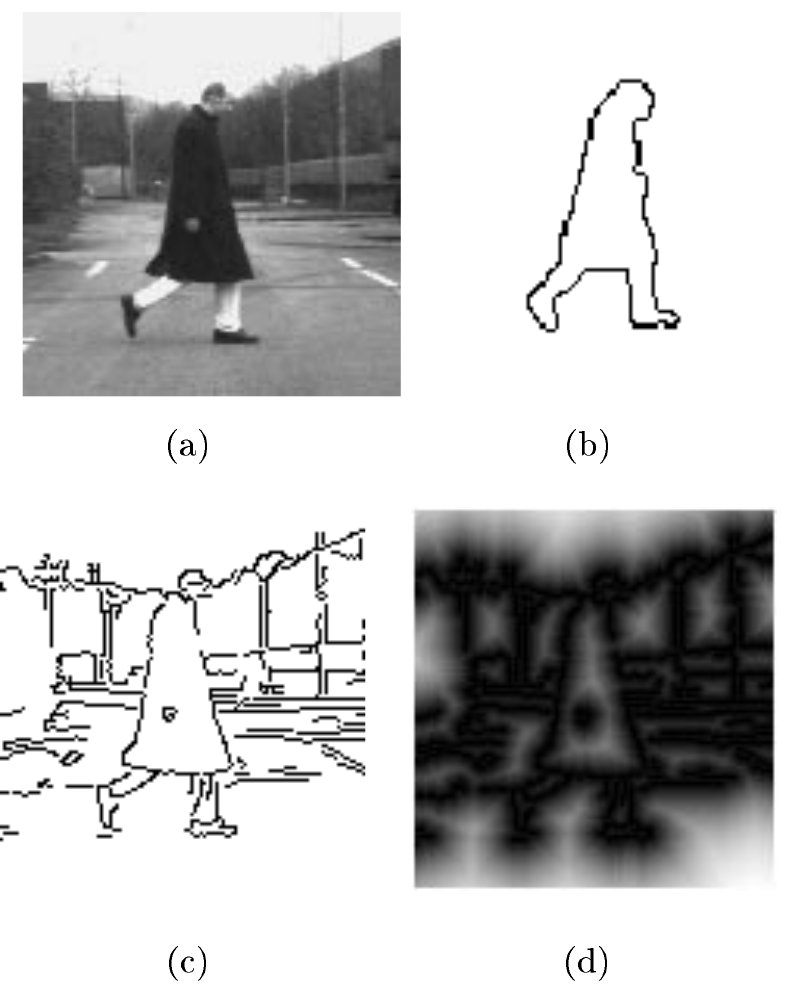
\includegraphics[width=0.6\linewidth]{pedestrian_detection.jpg}
\caption{a) původní obraz b) vzor c) nalezené hrany d) vyobrazené vzdálenosti
Převzato ~\cite{7} }
\end{figure}
V rámci optimalizace se tato metoda (jak překládat chemfer matching system??) rozšiřuje na hierarchizovanou, která sdružuje podobné vzory do shluků a tudíž se prohledávání databáze zrychlí (viz obrázek 4).
\begin{figure}[h]
\centering
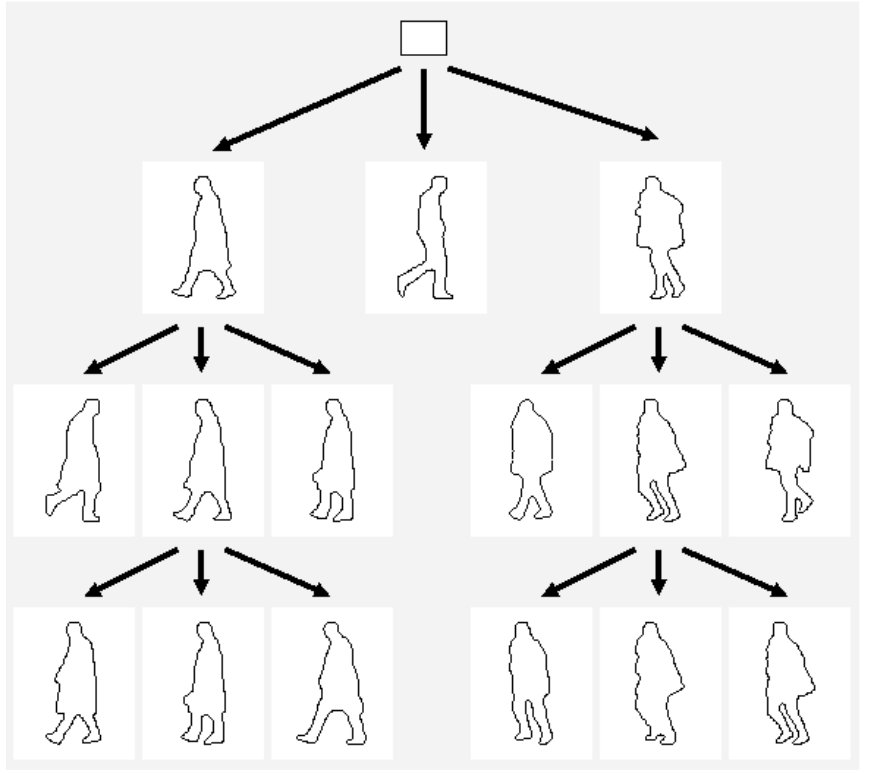
\includegraphics[width=0.6\linewidth]{hier.jpg}
\caption{Využití hierarchie v databázi vzorů. Převzato z ~\cite{7} }
\end{figure}
\newpage

Ověření výsledku probíhá RBF (radial basis functions) klasifikátorem. Nejdříve se z původního obrazu vybere čtyřúhelník obsahující možnou postavu a na základě euklidovské vzdálenosti určuje, jestli jednotlivé pixely jsou součástí postavy či nikoliv.\\
%RBF classifier!

Riggol a spol.~\cite{11} kombinují rozpoznávací metody založené na prvcích a na modelech za cílem dosažení spolehlivého a efektivního programu. Využívají P2DHMM (Pseudo-2D Hidden Markov Model). Jedná se o předem naučený algoritmus, který dokáže na základě pravděpodobností určit, jestli se jedná o postavu nebo ne. Příklad detekované postavy a postupné rozhodování je vidět na obrázku 5.\\
\begin{figure}[h]
\centering
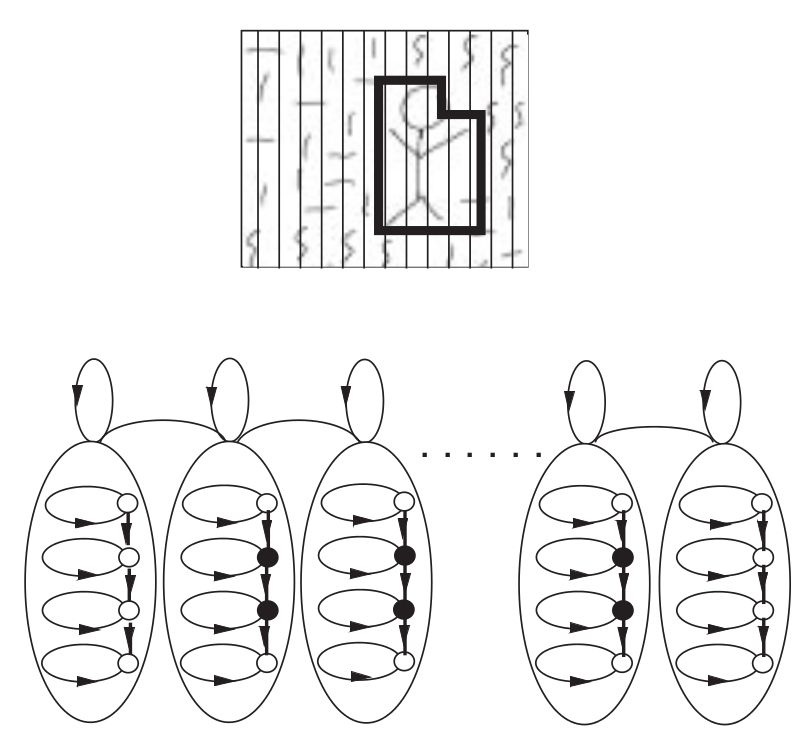
\includegraphics[width=0.5\linewidth]{P2DHMM.jpg}
\caption{Stochastický model 2D objektu. Převzato z ~\cite{11} } %stochastic model of 2D object using P2DHMM
\end{figure}


\subsection{Rozpoznávání částí těla}
%Hledání rukou na základě~\cite{10} :\\
%	vzhledu (barva, tvar)\\ 
%	naučené(learning based) -kNN,..\\
%			-Haar cascades\\
Ruka má 23 stupňů vlastností a v kombinaci s různým osvětlením a změnami v pozadí se jedná o značně komplikovaný problém na řešení pomocí podobnosti.\\

Jestliže aplikace nevyžaduje dynamické využití, lze použít rozdíl mezi objektem a pozadím~\cite{14}. Vyžaduje to co nejvíce neměnné pozadí a dostatečný rozdíl mezi objektem a zbytkem. Rozdíl lze hledat jednoduše procházením pole nebo využitím "chytrého" algoritmu. Spočívá v identifikaci čísti obrazu, která se hýbe oproti posledním obrazům. Příklad detekce ruky odstraněním pozadí je ukázán na obrázku 6.

\begin{figure}[h]
\centering
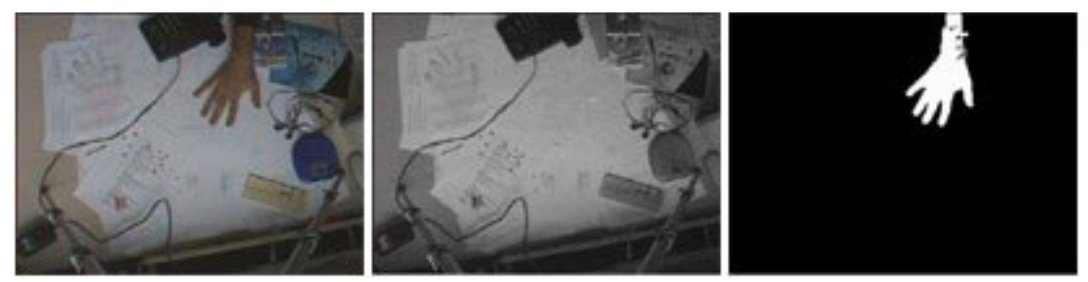
\includegraphics[width=1\linewidth]{diff.jpg}
\caption{a)vstup  b) referenční obraz  c)výstup 
Převzato z ~\cite{14} } 
\end{figure}


\subsection{Rozpoznávání gest}
Mezi rozpoznávání na základě vzhledu se řadí mnoho metod zahrnujících strojově naučené algoritmy jako neuronové sítě, HMM (Skrytý Markovův model) a jiné~\cite{3}. Gesto lze identifikovat i pomocí určení pozice a směru ruky a jednotlivých prstů.\\ %vyčetení/ identifikace?

Kim a spol.~\cite{5} používají bílé značky na špičkách prstů, které sledují černým světlem a detekují jednoznačně špičky prstů, což umožňuje velkou škálu možných gest. Na druhou stranu vzniká i omezení barvy pozadí, které lze eliminovat jen v určitém prostředí, tudíž se jedná o vhodnou variantu k využití při hrách ve VR (virtuální reality).\\

Shaker a Zliekha ~\cite{12} získávají směr prstu na ruce, kterou snímají dvěma kamerami. Jedna kamera natáčí shora, zatímco druhá zboku. Oba vstupy se zpracovávají zvlášť do rozpoznávání gesta. Nejdříve přepočítají obraz na stupně šedi a poté dle určené prahové hodnoty odfiltruje pozadí a vytvoří binární obraz. V tomto kroce je třeba, aby bylo pozadí jednoduché a jasně rozlišitelné od ruky. Kvůli odstranění šumu se obrázek rozmaže a následně zaostří. V tomto kroce vzniká podmínka, že největší objekt v obraze je právě ruka. Poté se pomocí Laplaciána získají hrany daného objektu a z něj se vytvoř kontury.
Gesto se identifikuje pomocí nalezení největšího vrcholu v obraze a nalezení čáry, kterou opisuje natažený prst a následnou kombinací obou směrů do 3D. Postup je znázorněný na obrázku 7.
\begin{figure}[h]
\centering
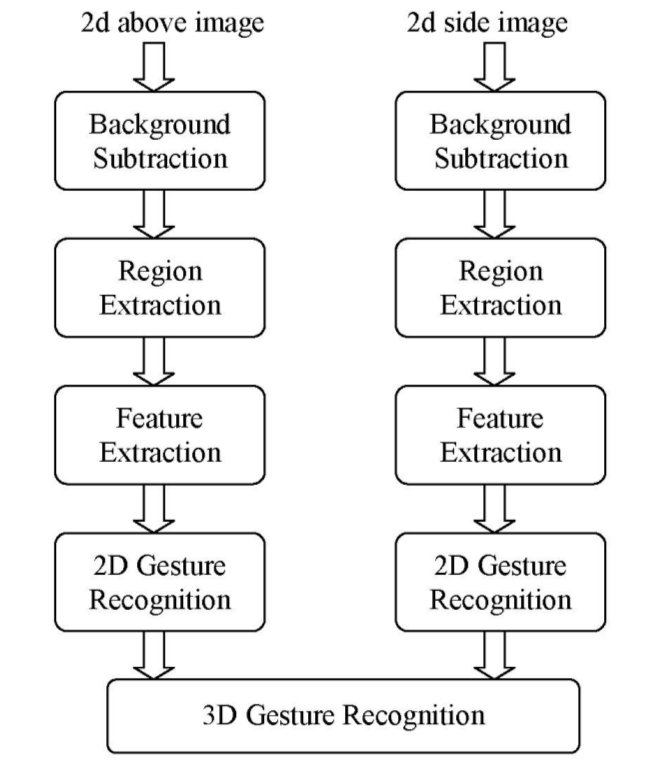
\includegraphics[width=0.5\linewidth]{ShZl.jpg}
\caption{Popis algoritmu. Převzato z ~\cite{12} } 
\end{figure}

\subsubsection{Rozpoznávání prstů}
Hackenberg a spol.~\cite{12} implementovali identifikaci prstů a dlaně na základě několika kroků. Nejprve projde hloubkový obraz z kamery a hledá tvary podobné špičkám prstů nebo rourovitého tvaru podobného prstům. Poté se zaměří na detailnější vlastnosti dlaně. Z nalezených vhodných polí, která mohou představovat dlaně se vyřadí ta, která nejsou napojena nijak na prsty, jsou menší než předem určená hodnota (odvozená od průměrně velikosti hlavy) a vzdáleností špiček prstů od dlaně.\\


Bez potřeby porovnávání tvarů a zdrojů se dají rozpoznat jednotlivé špičky prstů pomocí nalezení lokálního maxima v obrysu ruky. Ve všech adekvátních směrech se naleznou kandidáti a následně vyloučí mylné identifikace. Jedná se ale o postup náchylný k šumu v obraze, podobná metoda odolnější navrhuje porovnávání vzdálenosti obrysu k pozici ruky~\cite{3}.\\
Jednotlivé prsty lze rozpoznat například pomocí vyhledávání na základě tvaru~\cite{4}. Jde o zjednodušení představy objektu na geometrický objekt a vyhledávání vhodných kandidátů v obraze. 
%obrázek figertip jako geometrického objektu ze zdroje?

Mezi další programy rozpoznávající špičky prstů z již relativně čistého čtyřúhelníku, který obsahuje zájmový objekt, patří identifikace na základě dvou specifických vlastností. Centrum špičky je obklopen kolem pixelů patřící prstu a ten je obklopen dlouhou řadou pixelů nepatřících prstu~\cite{14}. Ruce lze identifikovat i až po prstech a to tak, že se vyloučí objekty podobného tvaru (propisky, fixy), které nesplňují vlastnosti rukou, například nepatří k žádné dlani.

\begin{figure}[h]
\centering
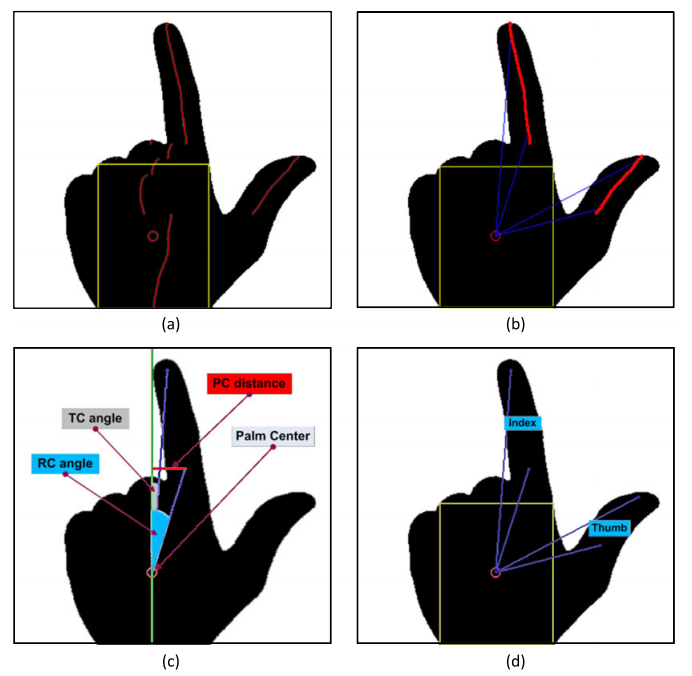
\includegraphics[width=0.5\linewidth]{fingers.png}
\caption{Vyobrazení definovaných pojmů, které lze využít k výpočtům pozic, na základě proporcionálních vlastností prstů.
Převzato z ~\cite{13} }

\end{figure}
\begin{center}
$RC_{angle} = 90 - tan^{-1} \frac{y_{r}-y_{pc}}{x_{r} - x_{pc}}$ \\
$TC_{angle} = 90 - tan^{-1} \frac{y_{ft}-y_{pc}}{x_{ft} - x_{pc}}$ 
\end{center}
\newpage
\section{Aktuální aplikace}
Všechny aplikace, které mohou využít výhod~\cite{14}:
\begin{itemize}
\item Ovládání na velmi malém prostoru
\item Ovládání z větší vzdálenosti
\item Snížený počet součástek
\item Zjednodušené ovládání elektroniky
\item Potenciál zabezpečení proti zneužití (při implementaci ochranných prvků)
\item Minimalistické (méně tlačítek a obdobných prvků)\\
\end{itemize}
Potenciál pro využití v:
\begin{itemize}
\item Překlad znakové řeči
\item Ovládání chytrých zařízení (chytrá domácnost - světla, hudba, televize, telefon)
\item Prezentace před publikem (ovládání počítače)
\\
\end{itemize}
Již využíváno v:
\begin{itemize}
\item Rozpoznání chodce v dohledu vozidla
\item Sociální experimenty (vyslání robota stopovat)
\item Ovládání a hraní na konzolích
\end{itemize}

\subsection{Konkrétní aplikace}
\subsubsection{Rehabilitace}
Mezi využítí v lékařské oblasti patří převážně rehabilitační cvičení. V nemocnici ve městě Reading využívají kameru Kinect pacienti po mrtvici na zlepšení pohyblivosti a koordinace~\cite{21}. 

\subsubsection{UI během operace}
Další možnosti se nabízí i při procházení záznamů pacienta při operaci, aniž by se kdokoliv dotýkal nesterilních věcí. Další možností se nabízí i na operačním sále, když chce doktor přístup k záznamům pacienta a nemusí se tak dotýkat žádných nesterilních věcí~\cite{24}.\\

//cite{22} preliminary investigation of movement

\subsubsection{Bixi}
Bixi je bezdotykový ovladač k mobilnímu zařízení. Hlavním zaměřením je usnadnění ovládání vedlejších aplikací během řízení auta tak, aby se řidič mohl soustředit na provoz. Po spárování se zařízením pomocí bluetooth lze gesty volit adresu pro navigaci, ztlišit či zastavit hudbu, ztlumit jas obrazovky, přijímat hovory a jiné.

\endinput
%%
%% End of file `ch01.tex'.

  \chapter{Implementace rozpoznávání gest}
Následné algoritmy byly testovány na Kinectu v2 pomocí projectGeneratoru od openFrameworks. Program má i vývojové prostředí, ze kterého to lze spouštět. V přiloženém README.txt bude uveden postup pro generátor pomocí příkazové řádky.

\section{Software}
\subsection{openFramworks}
OpenfFrameworks ~\cite{1} je open source C++ nástroj pro kreativní programování.\\
Využívá se doplněk ofxKinectV2~\cite{2}. Oproti zabudovanému ofxKinect je optimalizovaný pro aktuální openFrameworks (verze 0.9.0), je stabilnější, rychlejší a podporuje pro případné potřeby i více kamer.

Kód v openFrameworks se dělí do třech hlavních částí. Jedná se o setup(), update() a draw(). Sekce setup slouží pro počáteční nastavení programu, proměnných apod., update obsahuje výpočetní a aktualizační část a draw má na starosti vykreslování.

Program se snaží vykonávat všechny části tak často, jak to lze. V update i draw se může využít funkce ofGetElapsedTimef(), která vrací vteřiny v jednotkách float od spuštění programu nebo ofGetElapsedTimeMilis(), která vrací milisekudny od resetování čítače. Pomocí využití modulo funkce (i jiných) můžeme ovlivnit jak často se bude vykonávat každá aktualizační část nebo její podčást, jelikož lze předpokládat, že člověk nemění gesta rychleji, než je počítač zpracovává. Omezení snímků určených ke zpracování programem lze povést i pomocí funkce isFrameNew(), která vrací boolean hodnotu určující, jestli se snímek změnil či nikoliv.

% %\subsection{Měření času v OF}
%timeStart = ofGetElapsedTimef();
%	/*kód*/
%timeEnd = ofGetElapsedTimef();
% %diffTime = timeEnd - timeStart;

\section{Hardware}
\subsection{Kamera Kinect}
K implementaci této práce je využita kamera Kinect v2. Zdroje, ze kterých lze data využít k potřebám aplikace jsou RGB kamera s rozlišením 1920 x 1080 pixelů a kamera na snímání hloubky s rozlišením 512 x 424 pixelů.

Jedná se o relativně levnou a dostupnou kameru, která se v době zpracování této práce (začátek roku 2018) dá pořídit do tří tisíc korun.

\section{Zpracovatelné vstupy}

Obě kamery mohou poskytovat užitečné informace pro účely projektu. RGB kamera nabízí pole pixelů, kde každý má složky RGB (0 až 255). Lze využít v kombinaci s robustním programem, který by na základě barvy, tvarů a dalších vylučovacích prvků správně detekoval nejdříve ruku a poté i gesta. Jedná se o znatelně náročnější způsob.

Hloubková kamera poskytuje pole s hodnotami 0 až 255 dle vzorce pro výpočet vzdálenosti na základě doby letu infračerveného světla. Stupnice hodnot je klesající, to jest nejbližší objekty mají hodnotu 255. Ve vzdálenosti 3 metry hodnoty klesnou na 150. 

\begin{figure}[htp]
\centering
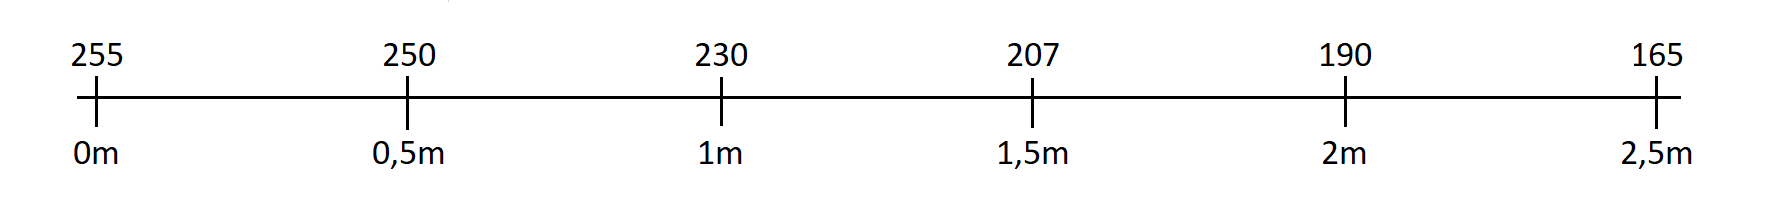
\includegraphics[width=\textwidth]{scale.png}
\caption{Stupnice hodnot, kterých nabývá hloubková kamera v závislosti na vzdálenosti}
\label{fig:scale}
\label{pic9}
\end{figure}

Minimální vzdálenost pro správné měření vzdálenosti je 0.5 m a maximální 4.5 m. Při větší vzdálenosti bude Kinect stále ještě detekovat věci v zorném poli, ale bude poskytovat nepřesná data a hloubková kamera pozbydu užitku. Velký vliv má i rozlišení, které je pro velké vzdálenosti nedostačující. V dálce 5 m od kamery je rozlišení 7 cm.

Využitelné parametry:

\begin{itemize}
\item Vzdálenost od kamery
\item Vzdálenost mezi pixely
\item Úhly
\item Barvy pixelů
\end{itemize}

\subsection{RGB video}
Výstupem z RGB kamery je dvoudimenzonální pole se třemi hodnotami jednotlivých barevných složek. Zpracování obrazu z RGB videa nebude v této práci implementováno, ale patří do jedné z variant, jak detekovat ruku a následně i gesta. \\

\subsection{Hloubkové video}
Zpracování hodnot z hloubkové kamery je jednodušší, už jenom protože se jedná o jednodimenzionální pole s hodnotami. Prahování (tresholding) se pak provádí jednoduchým porovnáním hodnot a vytvoření binárního obrazu je rychlejší.

Nedostatky vyplývající z využití pouze hloubkové kamery spočívají hlavně v tom, že pokud je v záběru objekt , který má podobnou stavbu a strukturu jako je ruka, tak je mylně detekován a zpracováván.

Doporučený postup by měl sestávat ze čtyř částí:

\begin{enumerate}
\item Úvodní nastavení
\item Nalezení ruky
\item Identifikace gesta
\item Vykreslení ruky (volitelné)
\end{enumerate}

\subsubsection{Úvodní nastavení}
Lze zde dát uživateli na vědomí podmínky interakce s kamerou. Například pozice ruky musí být v prostřední třetině. Alternativou může být počáteční umístění ruky doprostřed kamery, aby mohla dále vycházet z umístění za využívání historie nebo aby se zkrátila doba hledání ruky. V této aplikaci je nejen počátečná podmínkou, že ruka musí být nejbližší objekt před kamerou.

\subsubsection{Nalezení ruky}
Jedná se o prostor pro určení podmínek a způsobu vyhledávání ruky. Tato část rozhoduje o robustnosti kódu a využitelnosti aplikace. Je vhodné nejdříve odstranit nulové a jinak nevyhovující pixely, vyplnit díry v obraze a počítat s dalšími chybami hardwaru a vlivy okolí. Pokud má být aplikace využívaná v jakkoliv náročnějším okolí, musí obsahovat i vyloučení veškerých nevyhovujícíh objektů, jako jsou věci podobného tvaru či případně cizí ruce. Při využívání pouze czdáleností a úhlů jednotlivých pixelů se těžko zahrnují všechny možnosti a způsoby provedení gesta. Jelikož mají lidé různé dispozice rukou, to co je pro jednoho normální, může kazit správnou detekci ruky jiného jedince.

Předpoklad pro následující text je zpracování videa ohledně nulových pixelů. Měly by být ignorovány v rámci chybného vstupu. Zároveň platí, že čím více podmínek se uživateli na začátku předloží, tím jednodušší je nalezení ruky. 

U správně ukazovaného gesta se dá předpokládat stejná vzdálenost jednotlivých bodů od kamery. Mírné odchylky se dají buď zahrnout offsetem, který rozdíly v určitém rozmezí bude považovat za ekvivalentní. nebo vyloučit úplně, jelikož se dá předpokládat, že to nebude mít vliv na zpracování, pokud se jedná o krajní body. Aby byl program uživatelsky přívětivý, v programu je zvolena odchylka na zachycení těchto rozdílů.

V tomto programu se vychází z předem definované vzdálenosti, ve které je nalezen největší možný čtverec, který by představoval dlaň. Pro účely nalezení by muselo existovat pole pixelů, které by reprezentovalo dlaň, či případně podobný objekt, který by se následně vyloučil podle dalších kritérií. Nadále by byla dlaň definovaná středem nalezeného čtverce a šířkou.

Následuje vylučování mylných objektů podle toho, jak robustní program má být a v jak obtížném prostředí bude detekce probíhat. Tato část je předmětem budoucích rozšíření, jelikož se jedná o komplexní problematiku.

Nutnou podmínkou ruky je, že obsahuje prsty, které mají proporcionálně ke dlani určitou velikost a vzdálenost od středu dlaně. Jelikož známe střed nalezené dlaně, lze identifikovat i prsty, respektive konečky prstů. Ze začátku musí být známo jaké gesto bude ruka zobrazovat při inicializaci, aby se dala nalézt. Pro ilustraci bude rozebráno gesto se všemi prsty nataženými. 

Nejjednodušší metodou je nalezení lokálních maxim po šíři dlaně. Když se dlaň rozdělí na čtyři části a v každé se nalezne maximum po ose y (ose x pro horizontální polohu ruky), pro každý prst se změří vzdálenost špičky prstu od středu dlaně. Pokud se bude výrazně odchylovat od proporcí běžné ruky, bude nalezený objekt vyloučen.

Rafinovanější programy využívají tvorbu skeletonu pro sledování a identifikaci jak postavy, tak i ruky. Jedná se o postup nalezení kostí a jejich kloubů, které jsou reprezentovány čárami, což pak reprezentuje ruku (případně tělo). Jedná se o možný, ale náročnější a zdlouhavější postup.

\subsubsection{Identifikace gesta}
Výběr jednotlivých gest je vhodno prodiskutovat s jejich potenciálními uživateli a rozhodnout se mezi dynamickými a statickými gesty. Případně by obě možnosti šly kombinovat, ale byl by to zbytečně komplikovaný postup. Pro gesta dynamická je potřeba udržovat si v paměti minulé stavy a stanovit dobu, po kterou by bylo přijatelné pro uživatele provádět gesto a zároveň to nemohlo být zaměnitelné nebo mylně identifikované. Nejjednodušší je identifikovat gesta statická, kde s využitím souřadnic lze vypočítat počet prstů, a tak v základní verzi bude prostor pro minimálně pět variant, pokud se pro zjednodušení vyloučí zavřená pěst. V momentě, kdy bude program podporovat identifikaci jednotlivých prstů od sebe, je k dispozici variant hned více, než by kdy bylo třeba nebo by bylo zapamatovatelné pro uživatele.

Počet prstů lze vypočítat po správné identifikaci jednotlivých prstů, a jedná se o nejjednodušší způsob klasifikace gesta. Pro přesnost se lze opřít i o úhly a vzdálenosti mezi středem dlaně a špičkami prstů podle vzorců uvedených v kapitole 2.1.4 u obrázku 8.

Sledování gesta může také probíhat pomocí ukládání historie. Za předpokladu, že se člověk hýbe pomaleji, než se střídají snímky k analýze, lze procházet menší část pole, například jen okolí místa, kde se posledně nacházela ruka s prsty a kontrolovat změny, zda počet ukázaných prstů se zmenšil nebo zvětšil. K tomuto účelu by stále stačilo gesto definované počtem prstů bez závislosti na tom, o které konkrétně se jedná.

Otázkou je i jaký objekt má představovat gesto. Jedná-li se o číslo, je to nejjednodušší. Může to být ale i objekt, který obsahuje pět prstů, z nichž každý může být zvednutý nebo nikoliv. Pak je podstatně přehlednější implementace více než pěti gest. Identifikace je ale náročnější, jelikož každý nalezený prst se musí nejdříve identifikovat, poté aktualizovat objekt představující ruku před kamerou a porovnat s implementovanými gesty. 

\subsubsection{Vykreslení ruky}
Objekty se přes video vykreslují pomocí FBO ("frame buffer object"). Jedná se o buffery s objekty, které je třeba vykreslit. Reprezentují plátno, na které se pomocí pomocí příkazů 'begin()' a 'end()' vykreslují 3D objekty a jednou za snímek či méně často (podle požadavků) se vykreslí pomocí příkazu 'draw()'. Pro lepší přehled se můžou jednotlivé prsty (konečky prstů) zvýraznit koulí, zatímco celá ruka krychlí. Vykreslují se pouze základní objekty, které upřesňují nalezenou pozici rukou a prstů, aby nebylo potřeba udržovat v paměti přesné okraje ruky, které ani nejsou potřeba.

\section{Předzpracování}

Kvůli přehlednější práci s matematickými parametry obrazu se nejdřívnačte video, které je uloženo v 1D poli do 2D pole pro další zpracování.\\

\subsection{Filtrace}
Jelikož se do obrazu dostane značné množství chybných hodnot, je potřeba je nejdříve co nejvíce eliminovat. Za tímto účelem je použit medián z okolí. Kvůli překreslování aktuálních hodnot jsou pro dalš výpočty použita data z pole zrcadlícího originální data. Pro každý pixel je načteno okolí o požadované velikosti, které se seřadí podle velikosti a jako výsledná hodnota se vezme hodnota z prostřední pozice.\\

Velikost okolí by se měla vybrat empericky. Čím větší okolí, tím více je výsledek rozmazaný, ale zato obsahuje menší počet odchýlených hodnot, které by mohly narušit průběh zpracování. Pokud se vezme okolí malé, zůstane jich více, ale lépe se zachovají tvary. Na následujících obrázcích lze pozorovat rozdíl mezi okolím 9 (obrázek ~\ref{pic10}) a okolím 25(obrázek ~\ref{pic11}).\\

\begin{figure}[htp]
\centering
\fbox{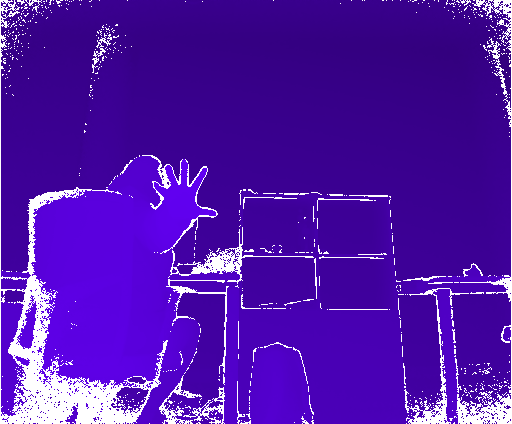
\includegraphics[width=.4\textwidth]{3-neigh9/befOUT.png}} \hfil
\fbox{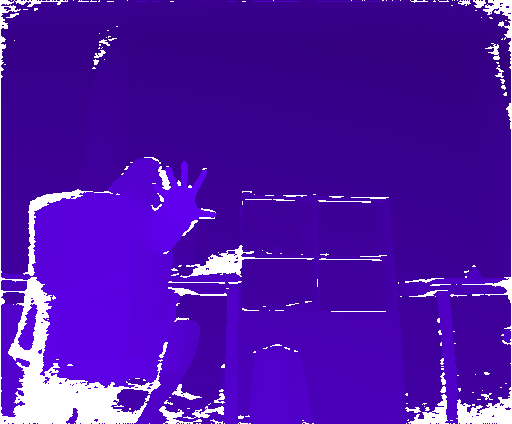
\includegraphics[width=.4\textwidth]{3-neigh9/afOUT.png}}
\caption{Medián vzatý z okolí mohutnosti 9 \\ a) originální obraz b) po úpravě}
\label{pic10}
\end{figure}
\begin{figure}[htp]
\centering
\fbox{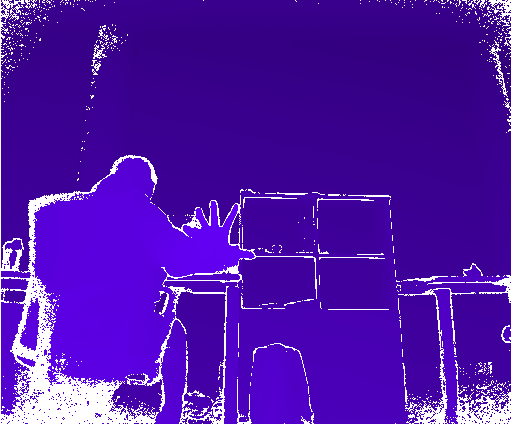
\includegraphics[width=.4\textwidth]{4-neigh25/befOUT.png}} \hfil
\fbox{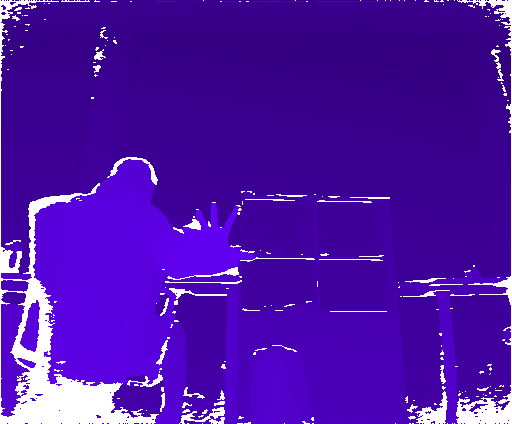
\includegraphics[width=.4\textwidth]{4-neigh25/afOUT.png}}
\caption{Medián vzatý z okolí mohutnosti 25 \\ a) originální obraz b) po úpravě}
\label{pic11}
\end{figure}

\subsection{Prahování}
Pro manipulaci s nalezenými tvary a výpočty mezi jednotlivými body je snazší pracovat s binárním obrazem. Nejdříve se obraz projde a najde nejbližší objekt (největší hodnota). Díky předchozí filtraci nezkreslí tuto hodnotu žádný špatně naměřený pixel. Následně se již porovná každý jednotlivý pixel s hodnotou a vytvoří se pole s hodnotami 1 a 0.

Jelikož lze předpokládat, že člověk nebude mít vždy ruku striktně kolmo k pohledu kamery, je záhodno odečíst od této hodnoty odchylku. Výsledná hodnota tedy záleží na tom, zda původní pixel byl blíže, než nejbližší objekt s ohledem na odchylku.\\
Na obrázcích ~\ref{pic12},~\ref{pic13} a~\ref{pic14} lze pozorovat změny s ohledem na různé tolerance naklonění ruky. S odchylkou 10 vidíme, že ještě kus dlaně chybí, při odchylce 15 je s rukou načtený i znatelný kus předloktí a k tomu i nejednotný kus jiného objektu. Při toleranci pouze 12 je stále načteno moc pixelů a tak se jeví 10 jako nejvhodnější tolerance.\\

\begin{figure}[htp]
\centering
\fbox{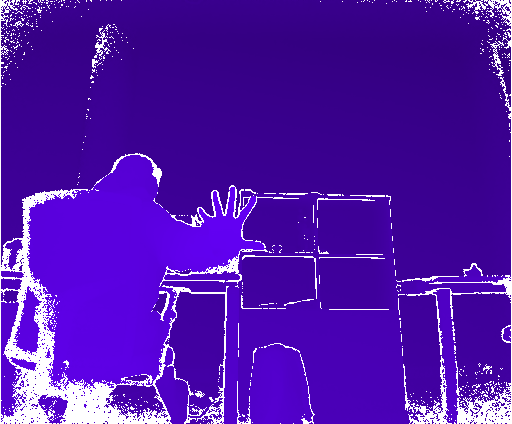
\includegraphics[width=.3\textwidth]{5-depth-10/befOUT.png}} \hfill
\fbox{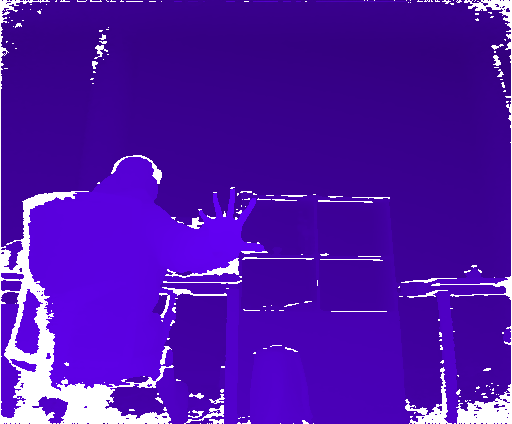
\includegraphics[width=.3\textwidth]{5-depth-10/afOUT.png}} \hfill
\fbox{
\includegraphics[width=.3\textwidth]{5-depth-10/binOUT.png}}
\caption{Prahování s odchylkou 10 \\ a) originální obraz b) po filtraci c) binární obraz}
\label{pic12}
\end{figure}
\begin{figure}[htp]
\centering
\fbox{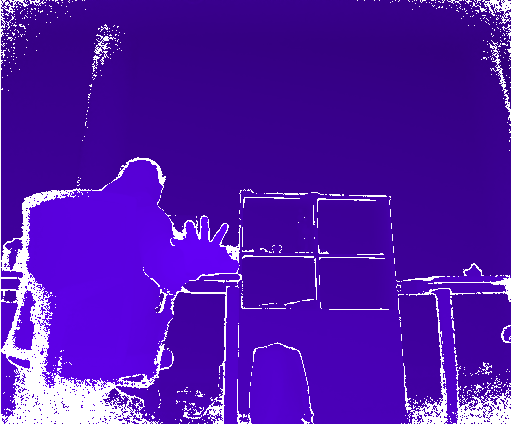
\includegraphics[width=.3\textwidth]{7-depth-12/befOUT.png}} \hfill
\fbox{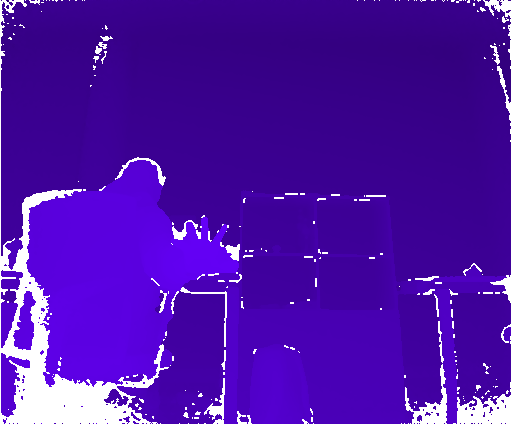
\includegraphics[width=.3\textwidth]{7-depth-12/afOUT.png}} \hfill
\fbox{
\includegraphics[width=.3\textwidth]{7-depth-12/binOUT.png}}
\caption{Prahování s odchylkou 12 \\ a) originální obraz b) po filtraci c) binární obraz}
\label{pic13}
\end{figure}
\begin{figure}[htp]
\centering
\fbox{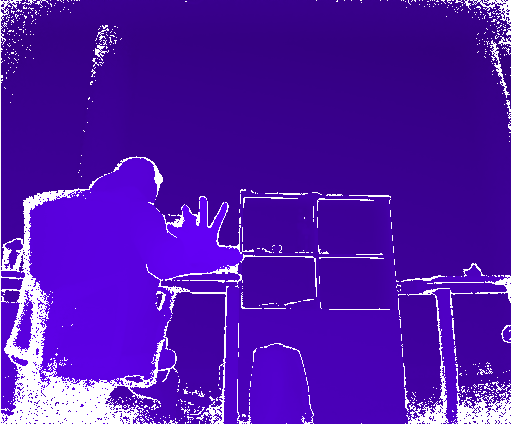
\includegraphics[width=.3\textwidth]{6-depth-15/befOUT.png}} \hfill
\fbox{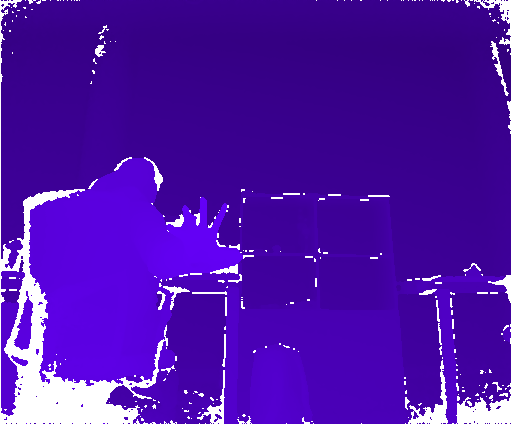
\includegraphics[width=.3\textwidth]{6-depth-15/afOUT.png}} \hfill
\fbox{
\includegraphics[width=.3\textwidth]{6-depth-15/binOUT.png}}
\caption{Prahování s odchylkou 15 \\ a) originální obraz b) po filtraci c) binární obraz}
\label{pic14}
\end{figure}
\newpage
\section{Detekce ruky}
Definujeme-li ruku jako nejbližší objekt, pak již při prahování je nalezena. Pro lepší názornost se ukládá umístění objektu pomocí pole souřadnic. Na videu je vizualizován pomocí červeného čtverce, který má střed v zprůměrovaných souřadnicích (Xavg, Yavg) a velikost odvozenou od velikosti pole. 
Na následujících obrázcích je vidět rozdíl mezi vyhledáváním v originálních datech a nebere v potaz chybné hodnoty a vyhledáváním v binárním obraze s vyfiltrovaným šumem.
\begin{figure}[htp]
\centering
\fbox{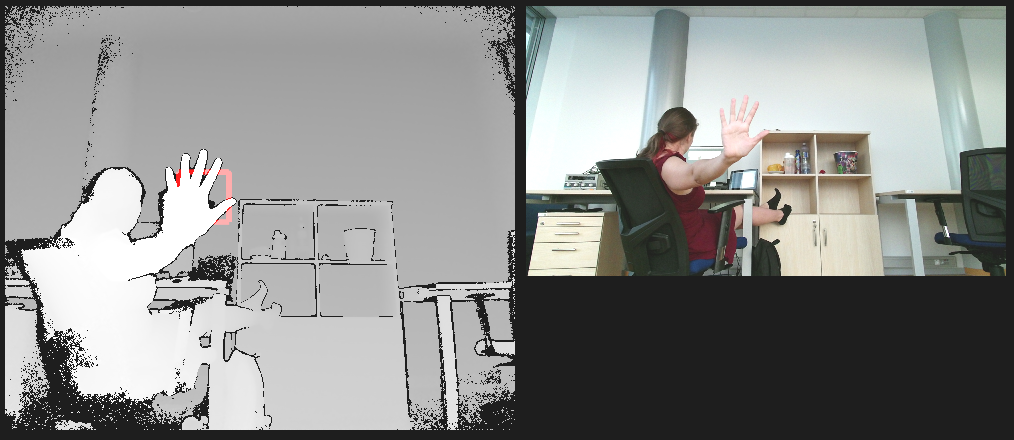
\includegraphics[width=.8\textwidth]{inDepth.png}}
\caption{Obrázek ukazuje největší nalezený nejbližší objekt z originálních dat.}
\label{pic15}
\end{figure}
\begin{figure}[htp]
\centering
\fbox{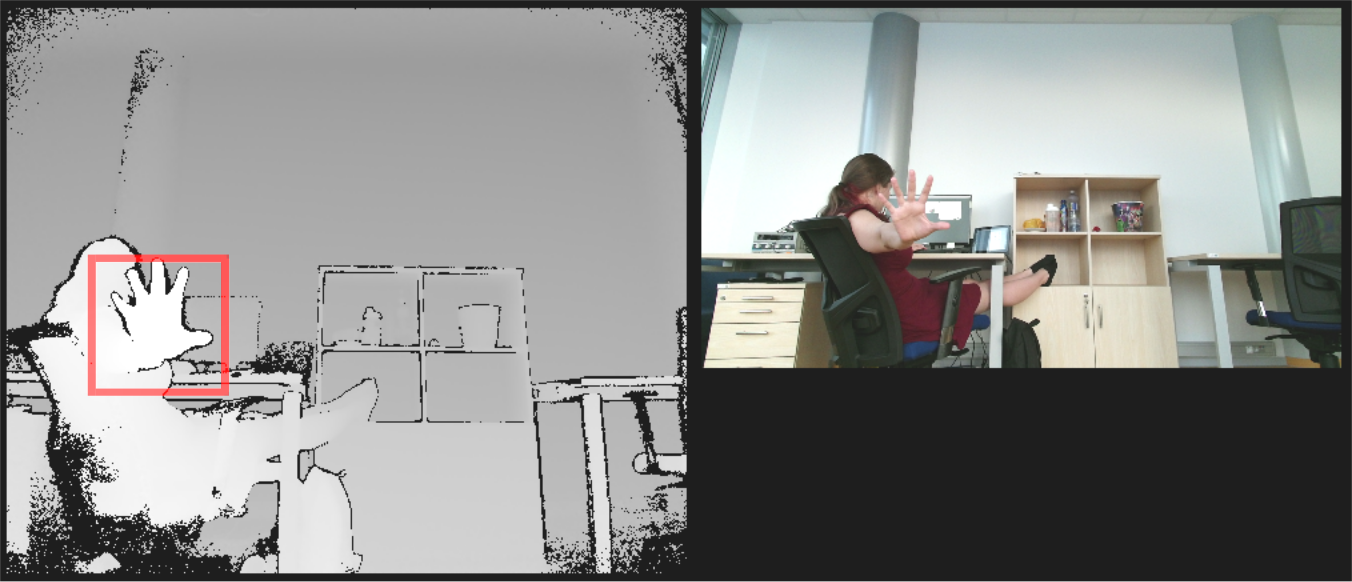
\includegraphics[width=.8\textwidth]{inBinary.png}}
\caption{Největší nejbližší objekt nalezený v binárních vyfiltrovaných datech.}
\label{pic16}
\end{figure}

Již z obrázků~\ref{pic15} a ~\ref{pic16} lze poznat, že vyhledávání v binárních datech je přesnější.
\newpage
\section{Detekce dlaně}
V binárním obraze se vyhledá největší čtvercová matice, kterou lze považovat za dlaň. Vytvoří se pomocná matice, do které se zapíší krajové hodnoty binárního obrazu a poté se binární pole prochází z levého horního rohu. Pokud je na dané pozici binárního obrazu nula, přepíše se i do matice. Pokud je tam ale jedna, pak se nalezne minimum třech sousedů z levého horního rohu. To znamená minimum z horního, levého a šikmo horního nalevo. K minumu se přičte jednička, čímž se zvětší velikost čtvercové matice. Ve výsledku tak největší číslo, které je nalezené v pomocné matici, představuje pravý dolní roh největší nalezené matice a zároveň její velikost~\cite{23}. Pro lepší práci v budoucnu je dlaň uložená jako středový bod a velikost matice.

\begin{figure} [htp]
%\begin{subfigure}[b][0.2\textwidth]
\centering
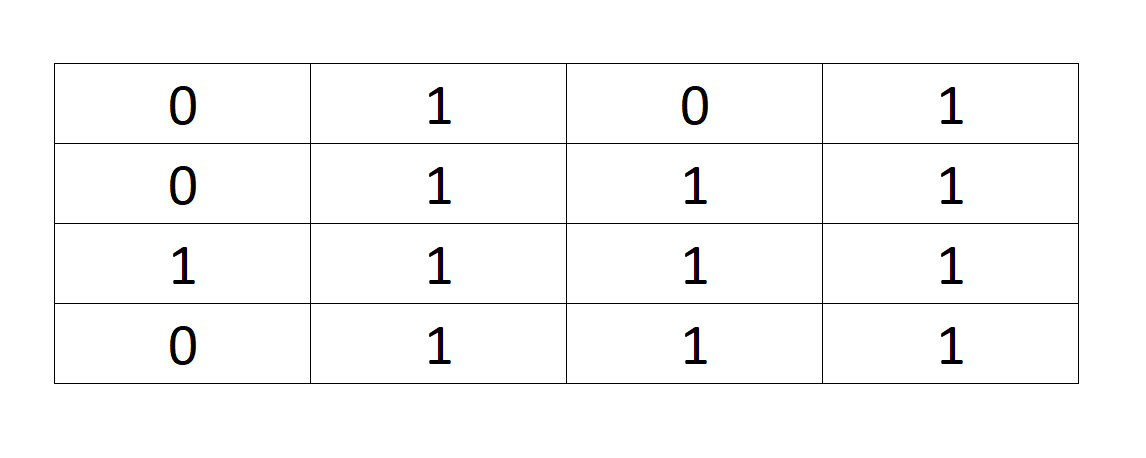
\includegraphics[width=.45\textwidth]{before.png} \hfill
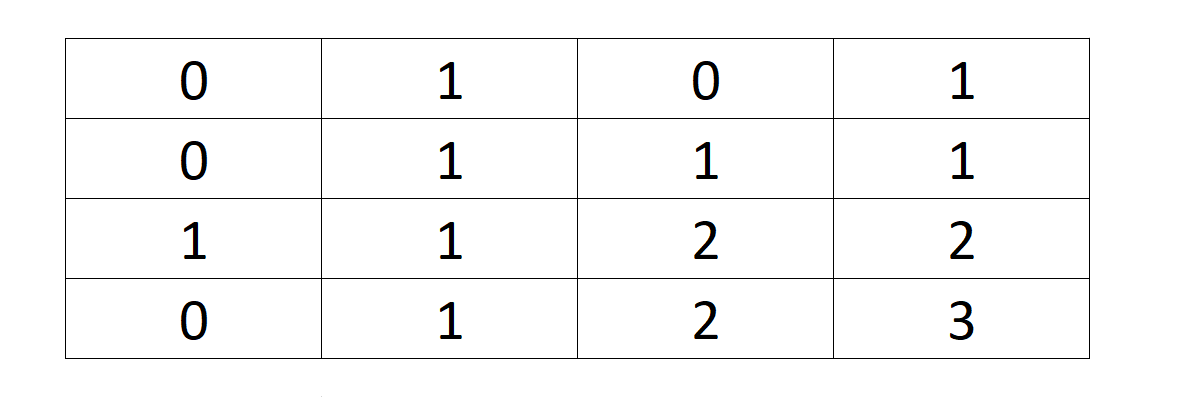
\includegraphics[width=.45\textwidth]{after.png} 
%	\caption{a) původní matice}
%\end{subfigure}
%\begin{subfigure}[b][0.2\textwidth]
%\caption{b) výsledná matice}
%\end{subfigure}
\centering
\caption{Nalezení největší jednotkové matice v binárním obraze.}
\label{pic17}
\end{figure}

Dlaň se vykresluje pomocí zeleného čtverce, jenž má velikost nalezené jednotkové matice a jeho střed má souřadnice Xc, Yc, které budou následně využívány jako střed dlaně.

\begin{figure}[htp]
\centering
\fbox{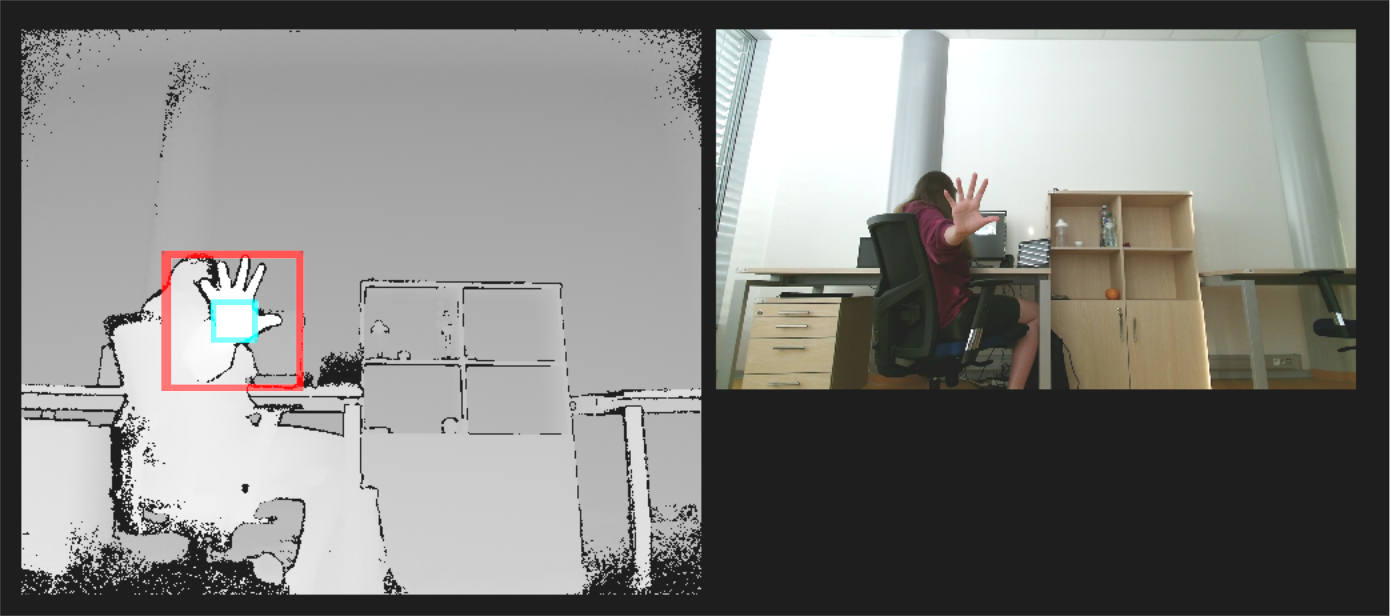
\includegraphics[width=0.8\textwidth]{square.png}}
\caption{Červený čtverec znázorňuje polohu a velikost nalezeného nejbližšího objektu.\\
Zelený čtverec obkresluje největší nalezený čtverec v objektu.}
\label{pic18}
\end{figure}

\section{Oblast zájmu (ROI)}
Pro optimalizaci algortimu se z původního obrazu vykrojuje ROI ("region of interest"). Po nalezení dlaně se z binárního obrazu překopíruje do menšího pole oblast okolo centra dlaně a všechny následující vyhledávání a detekce probíhá na již menším poli. 


\section{Detekce prstů}
V aplikaci je implentováno několik způsobů nalezení prstů. Ne všechny jsou efektivní a od některých se upustilo (viz kapitola statistika), ale pro různost postupu jsou zde uvedeny. Pro všechny platí předchozí úpravy obrazu a detekce směru prstů.

\subsection{Detekce směru prstů}
Za předpokladu, že jsou prsty nezaměnitelně hubenější, než předloktí, lze okolo dlaně ve vzdálenosti $ offset\_palm $ od okraje vést čáru ve všech čtyřech směrem (viz obrázek 19). Následně se iteruje podél jednotlivých čar a detekují změny v binárním obraze. Pokud jednotlivý nalezený objekt má šířku větší než je třetina šířky dlaně, jedná se o kus předloktí a nezapočítává se. Zbylé objekty se zaznamenávají do počtu předpokládanách prstů.  Pro přesnější detekci se daný algoritmus provede ještě jednou pro větší vzdálenost od dlaně. Pokud je pro obě vzdálenosti počet detekovaných prstů větší, než nula, je daný směr zaznamenán. Jelikož je potřeba znát i pozici palce, ukládají se dva směry prstů.

Empiricky nalezená nejlepší hodnota pro $ offset\_palm $ je $ \frac{5}{7} $ šířky dlaně, v druhém kole je zvolen dvojnásobný offset. 

\begin{figure}[htp]
\centering
\fbox{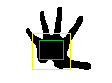
\includegraphics[width=.4\textwidth]{whereFingersAt.png}}
\caption{Zelený čtverec představuje hranice nalezené dlaně. Procházením podél žluté čáry, která je posunuta o offset se počítá počet změn a kontroluje tloušťka nalezených objektů. Pokud tlouťka odpovídá méně než třetině šířky dlaně, pak se považuje za prst.}
\label{pic19}
\end{figure}
\newpage
\subsection{Detekce konců prstů}
Všechny postupy se zakládají na prohledávání v okolí dlaně. Maximální délka prstů se odvozuje od nalezené velikosti dlaně. Prsty nesmí být ani příliš dlouhé ani příliš krátké.\\

%findFingerTips
\subsubsection{První metoda}
Nejjednodušší postup spočívá v rozdělení strany, na které se nachází prsty, na čtyři části, kde každá náleží jednotlivým prstům. Rozdělení je rovnoměrné a nepodporuje tak extrémní odchylky. Celkový obdélník musí být širší než dlaň a nebere se v potaz, který prst je v daném obdélníku nalezen. To znamená, že pokud se ukazují dva prsty, přičemž se některý/oba nachází ve vedlejším obdélníku, zaznamená se správně pouze počet prstů.

Jednotlivé části se následně procházejí a hledá se pixel, který ještě patří prstu a je nejvýše/nejníže dle orientace.\\

\begin{figure}[htp]
\centering
\fbox{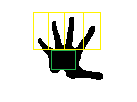
\includegraphics[width=.4\textwidth]{findFingerTips.png}}
\caption{Zelený čtverec představuje nalezenou dlaň. Žluté obdélníky jsou předpokládané pozice prstů na základě nalezeného směru.}
\label{pic20}
\end{figure}

%findFingerTips2
\subsubsection{Druhá metoda}
Další způsob zvyšuje použitelnost předchozí metody. Stále se prochází pole, ale celkový obdélník se předá v kuse a hledá se největší vzdálenost od středu dlaně. Stále platí omezení délky, tudíž je přesnější největší možná vzdálenost, která stále patří prstu.

%findFingerTips3
\subsubsection{Třetí metoda}
Funkce findFingerTips3 si ukládá souřadnice, na kterých byly detekovány prsty z předchozí kapitoly. Následně si dopočítá střed prstu a po přímce prohledává binární obraz tak daleko, dokud nenarazí na konec prstu (nulu v binárním obraze). 

%findFingerTips4
\subsubsection{Čtvrtá metoda}
Další implementovaná možnost nalezení konců prstů spočívá v procházení oblasti, ve které se nachází prsty. Hledání začíná u vnější strany a jakmile se narazí na pixel patřící objektu, uloží se jeho pozice a souřadnice se zapíše do pomocného pole. Pole obsahuje souřadnice, na kterých se nachází již nalezené prsty a navíc jejich okolí, ve kterých se stále jedná o ten stejný prst. Při následujícím nalezení pixelu patřícího k objektu se tedy nejdříve zkontroluje, jestli se nejdná o kolizi z pohledu již nalezených prstů.


\section{Statistika}
Vyhodnocení funkčnosti a použitelnosti navržených metod.

\endinput
%%
%% End of file `ch01.tex'.

  \chapter{Závěr}
Vybraný postup implementace zaručil určité výhody oproti jiným algoritmům. Mezi hlavní výhody paří, že nejsou potřeba žádné jiné věci, než je kamera. Člověk ovládající robota nemusí  být oproti žádnému konkrétnímu pozadí, nemusí mít na rukou rukavice nebo mít jiné specifické náležitosti. Úvodní kalibrace také není nutná. 

%možnosti budoucího využití
Jelikož je rozpoznávání vykonáváno v binárním obraze, je možná kombinace více programů nebo metod relativně jednoduchá. Zároveň lze program použít i s jinými hloubkovými kamerami. Pokud se algoritmus zkombinuje s využíváním obrazu z barevné kamery, dalo lze detekci provádět spolehlivěji.
Do programu lze také přidat nová gesta, odstranit stávající nebo změnit celkový pohled, na základě kterého se definují gesta. To lze udělat z pohledu přesnějšího rozpoznávání, tak i z pohledu, jak se jednotlivá gesta uvažují (počet prstů versus konkrétní prsty). 
%zhodnocení výsledků
%odůvodnění proč a jak

TODO zhodnocení výsledků - statistiky


\endinput
%%
%% End of file `ch01.tex'.


  %\startAppendices
  %  \include{app01}
  %\stopAppendices
\stopBodyMatter

\startBackMatter
  \PrintBibliography
  %\PrintIndex % define index entry in the text by: \index{word}
\stopBackMatter

\end{document}

\endinput
%%
%% End of file `template.tex'.
